\chapter{Designs and Performance Modeling}

Two CNN models - GoogLeNet (inception V1) and Resnet-50 - were implemented on FPGAs in the project. The choices were made based on :  
\begin{itemize}
  \item complexity of CNN models
  \item relevance in the industry
  \item accuracy of the models
  \item availability of pre-trained weights and biases
  \item project timeline
\end{itemize}  
We wanted to implement CNN models complex enough to require scaling over multiple FPGAs. This requirement was a direct consequence of our initial objective of wanting to scale over multiple FPGA devices. Here, the complexity of the model refers the number of hidden layers present in the model. GoogLeNet - with  xyz\todo{Add layer count} layers - and Resnet - with abc \todo{Add layer count} layers- are deep enough to warrant using multiple devices for implementing them.

As the winners of Imagenet Large Scale Visual Recognition Challenge(ILSVR) 2014 and 2015 respectively, GoogLeNet and Reset are quite well known in the industry. With an inference accuracy nearing human capability - GoogLeNet or exceeding human capability -Resnet-152, these models are very popular in the machine learning community. 

Since our objective was to implement an inference engine and not training an inference engine , it was imperative to work with models for which weights and biases were readily available. The popularity of GoogLeNet and Resnet in the machine learning community meant that the weights and biases were available freely in the form of frozen models \todo{Explain frozen models?}.

We stopped at two models as the time required to implement more models was significant and would have forced us to spend less time on other important tasks. And the main objective of our project - implementing CNNs on FPGAs - was met when we successfully implemented GoogLeNet and Resnet. We felt no additional findings would come out of implementing another CNN model on FPGAs.

Implementation of such complex applications on FPGAs calls for "Performance Modeling". Performance Modeling entails the detailed study of how kernels get executed on FPGAs. Performance Modeling allows a design engineer to understand the bottlenecks, performance limiting issues, general performance etc of kernels. Using performance modeling and making an educated assumption about the final design clock frequency, a design engineer can also predict the approximate run-time of a design.
For all the designs which we implemented, we also created models to explain the performance of our designs.    

In the next few sections, we explain in detail how we implemented different FPGA designs of GoogLeNet and Resnet-50 and the accompanying performance models.



\section{GoogLeNet}

The first CNN model we implemented was GoogLeNet. The idea of multiple designs of GoogLeNet was hatched to see the difference in performances when different levels of optimizations are applied at OpenCL level and architectural level. 
We were able implement three major designs for GoogLeNet :
\begin{itemize}
  \item Baseline
  \item DSP Usage Optimized
  \item Hybrid Design
\end{itemize}  

\subsection{GoogLeNet Baseline}

GoogLeNet Baseline was implemented by modifying the OpenCL code generated by TVM for GoogLeNet. We modified the generated code to meet the requirements of our plugin. Some of the major modifications which were performed are :
\begin{itemize}
  \item renaming kernel names
  \item merging ReLUs with Convolutions
  \item rewriting Concatenation layers to support NCHW layout
  \item removing transpose kernels
\end{itemize}  
We had to rename kernels as the naming convention used by TVM and our plugin was not the same. We  had to make sure that we had all the kernels in OpenCL code that the plugin expected to launch.

By merging ReLUs with Convolutions, we optimized away the need to send data from one kernel(Convolutions) to another(ReLUs). This preoptimization step is used in the Deep Learning Community widely as ReLUs are basically light weight operations and do not warrant a separate kernels.

By analysing our plugin, which is an extension to OpenVINO, and TVM, we realized that the layout used by OpenVINO and TVM were quite different. OpenVINO uses NCHW layout scheme whereas TVM uses NHWC layout scheme in Concatenation layer and NCHW layout scheme in all the other layers. To convert from NHWC to NCHW, TVM had generated transpose kernels. We modified all the Concatenation kernels to output NCHW thereby eliminating the need to have transpose layers.  

The modified code was first compiled to run on an FPGA emulator \todo{Insert correct name for emulator}. We verified the functional correctness of the modified code by comparing the values output by our modified code with the values output by TensorFlow implementation of the same model.  

The initial reports generated for this modified OpenCL code indicated that this implementation of GoogLeNet was far too big to fit on a single Stratix 10 board. In order to successfully run this design on FPGAs, there was a need to divide the design into smaller parts. By dividing the design into 10 smaller parts, we took advantage of the inherent logical divisions present in GoogLeNet topology. As  described in \ref{GoogLeNet_Topo}, every inception module is followed by a  Concatenation layer. Thus, we divided our design into ten smaller parts.  The first part is a purely feed forward design. The rest of the parts contain at least one inception module each and other layers as shown in Figure \ref{fig:GoogLeNet_division}


\begin{figure}[h!]
  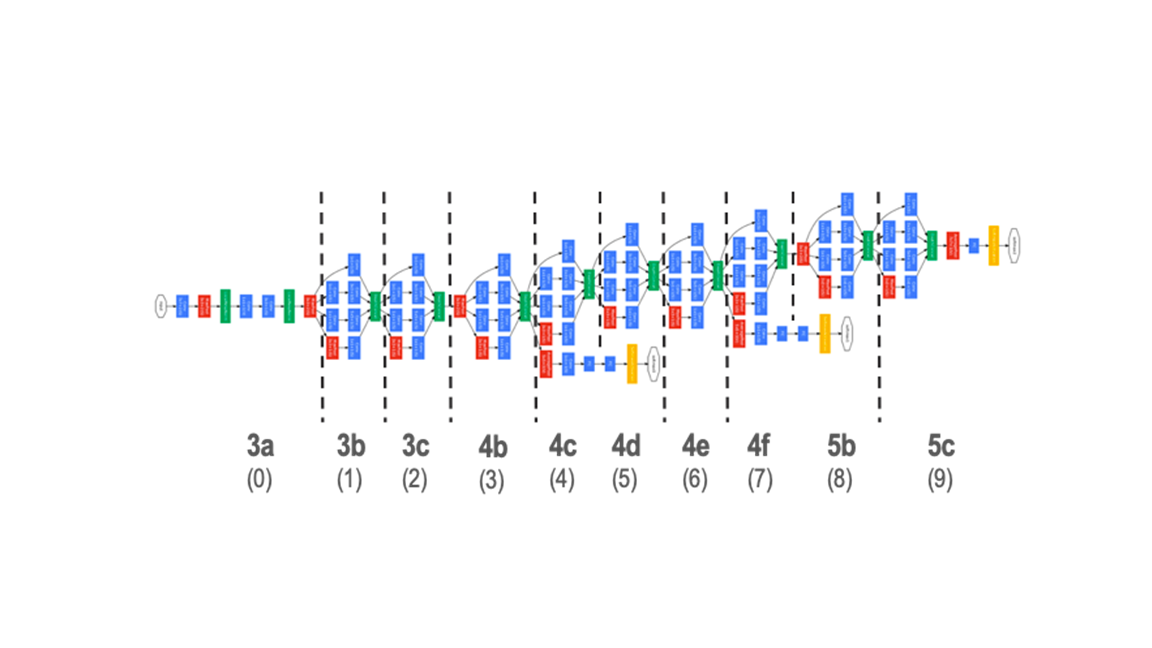
\includegraphics[width=\textwidth,height=\textheight,keepaspectratio]{img/GoogLeNet_division.png}
  \caption{Division of GoogLeNet topology}
  \label{fig:GoogLeNet_division}
\end{figure}
 
The 10 resulting OpenCL bitstream files (in aocx format) were named as "inceptionX", where X represents the ordinal value(shown in brackets) of the part the file is made of as shown in Figure \ref{fig:GoogLeNet_division}. For example, the file containing the description of part 3a in Figure \ref{fig:GoogLeNet_division} was named as "inception0.aocx". This naming convention plays a crucial part in deciding the order in which the bitstreams are flashed on multiple devices as discussed further ahead in this section.  


















\subsection{GoogLeNet DSP Usage Optimized}
\subsection{GoogLeNet Hybrid Design}

\section{ResNet}
\subsection{ResNet Baseline}
\subsection{ResNet Opt-V1}
\subsection{ResNet Opt-V2}
\subsection{ResNet Opt-V3}
%End of the chapter